\chapter{Полученнные результаты}\label{chap1}

%%%%%%%%%%%%%%%%%%%%%%%%%%%%%%%%%%%%%%%%%%%%%%%%%%%%%%%%%%%%%%%%%%%%%%%%%%%%%%%%
\section{Обзор библиотеки gym}\label{1sec:optimal-control}
%%%%%%%%%%%%%%%%%%%%%%%%%%%%%%%%%%%%%%%%%%%%%%%%%%%%%%%%%%%%%%%%%%%%%%%%%%%%%%%%

Для решения исходной задачи используется библиотека gym, в которой имеется ее реализация. Библиотека gym -- это open-source набор инструментов для разработки и сравнения алгоритмов обучения с подкреплением. Данная библиотека не делает никаких предположений о структуре агента и совместима с любой библиотекой численных вычислений, такой как TensorFlow или Pytorch. В ней собраны и реализованы классические задачи оптимального управления и несколько игровых задач. 

Сама библиотека симулирует среду. Таким образом агент может подавать в среду действие, а на выходе получать награду и состояние среды. Самый простой способ запустить ее вызов на 1000 шагов с выбором случайного действия из набора всех возможных действий представлен ниже. 

\begin{minted}[mathescape, linenos]{python}
import gym 
env = gym.make('Pendulum-v0')
env.reset() 
for i in range(1000): 
    env.render() 
    env.step(env.action_space.sample()) # take a random action 
env.close()
\end{minted}

Таким образом \mintinline{python}{env} -- это непосредственно среда. Для сброса ее в начальное состояние используется команда \mintinline{python}{env.reset()}. \mintinline{python}{env.redner()} рисует картинку полученного состояния текущей среды. Пример можно найти на рисунке 4.1. Множество всех доступных действий можно найти с помощью команды \mintinline{python}{env.action_space}. Чтобы совершить действие нужно вызвать команду \mintinline{python}{env.step(action)} и передать в него необходимое действие (\mintinline{python}{action}). В ответ на это среда вернет четыре параметра \mintinline{python}{(observation, reward, done, info)}. Которые обозначают следующее:
\begin{itemize}
	\item observation -- состояние среды, наблюдаемое после совершенного действия.
	\item reward -- полученная награда от совершенного действия.
	\item done -- завершена ли текущая задача.
	\item info -- вспомогательная информация, используемая для отладки. 
\end{itemize}
 \newpage



\begin{figure}[!h]
	\caption {Пример обратного маятника}
	\centering
	\includegraphics[scale=1.2]{download.png}
	\label{fig:agent}
\end{figure}



%%%%%%%%%%%%%%%%%%%%%%%%%%%%%%%%%%%%%%%%%%%%%%%%%%%%%%%%%%%%%%%%%%%%%%%%%%%%%%%%
\section{Формулировка поставленной задачи оптимального управления}\label{1sec:optimal-control}
%%%%%%%%%%%%%%%%%%%%%%%%%%%%%%%%%%%%%%%%%%%%%%%%%%%%%%%%%%%%%%%%%%%%%%%%%%%%%%%%

В данной работе рассмотрим задачу оптимального управления неустойчивой системой — маятник. Состояние маятника задается одной координатой: 

\begin{itemize}
    \item угол отклонения маятника от вертикальной оси ($\phi$)
\end{itemize}

Для решения задачи использовалась библитека gym, в которой маятник выглядит как на рисунке 4.2. \newpage

\begin{figure}[!h]
\caption {Маятник}
	\centering
	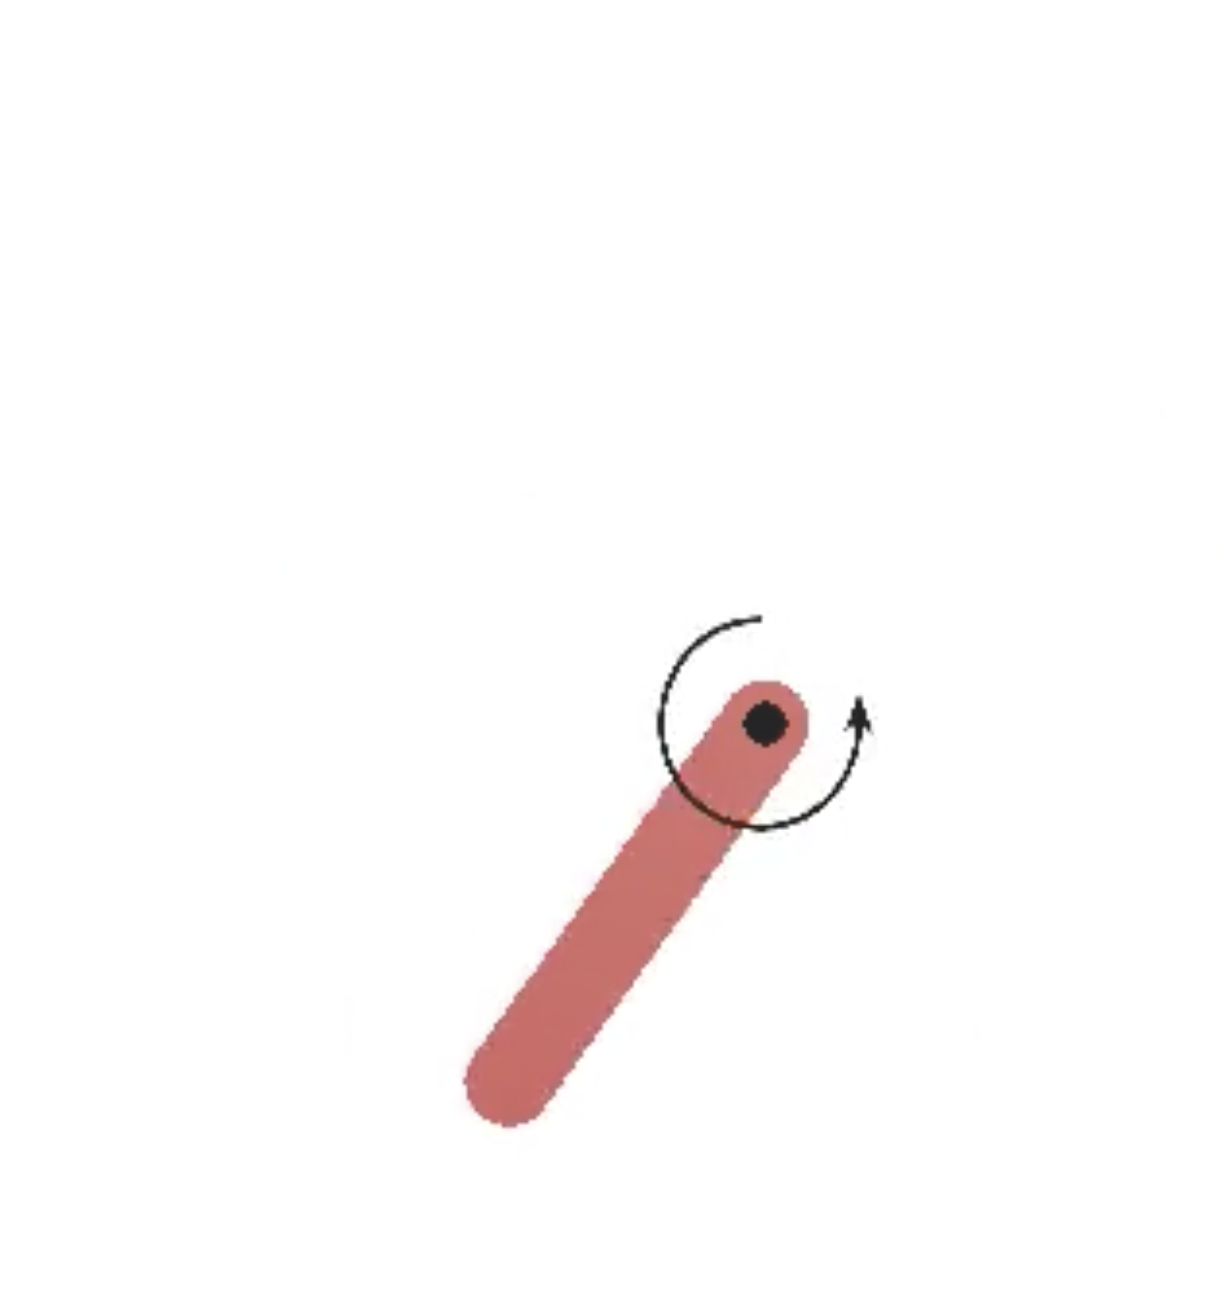
\includegraphics[scale=0.4]{pend.png}
	\label{fig:agent}
\end{figure}


На переменную накладываются следующие ограничения:
\begin{equation}
	\begin{aligned}
		\phi_{min} \leq \phi_k \leq \phi_{max} \\
		k = \overline{0, N-1}.
	\end{aligned}
\end{equation}

В нашем случае вводятся следующие ограничения:
$\phi_{min} = -115$,  $\phi_{max} = 115$. 
Кроме того рассматриваются два управления (действия): $u = \pm 1$, то есть либо толкнуть маятник вправо, либо влево.

За каждое действие, после которого маятник находится в вертикальном положении дается награда в 1 балл. Цель задачи -- при 200 запусках сессий  привести маятник в вертикальное положение и в конце получить среднюю награду хотя бы в 0.



Для решения задачи при подсчете $q(s, a)$ использовалась следующая архитектура нейронной сети: 
\begin{figure}[!h]
\caption {Архитектура сети}
	\centering
	\includegraphics[scale=0.45]{nn1.png}
	\label{fig:agent}
\end{figure}
 

\newpage

%%%%%%%%%%%%%%%%%%%%%%%%%%%%%%%%%%%%%%%%%%%%%%%%%%%%%%%%%%%%%%%%%%%%%%%%%%%%%%%%
\section{Результаты q-обучения}\label{1sec:optimal-control}
%%%%%%%%%%%%%%%%%%%%%%%%%%%%%%%%%%%%%%%%%%%%%%%%%%%%%%%%%%%%%%%%%%%%%%%%%%%%%%%%

Для того, чтобы наш алгоритм мог находить новые действия к уже имеющемуся алгоритму q-learning добавилась политика $\epsilon-gready$. Это значит, что на каждой итерации с вероятностью в $\epsilon$ вместо лучшего действия может быть выбрано рандомное. На каждой эпохе обучения мы запускам 100 сессий и считаем среднюю полученную награду. 

В итоге уже после 18 эпох мы достигли необходимого количества действий. График обучения представлен на рисунке 4.4.

\begin{figure}[!h]
\caption {График обучения модели}
	\centering
	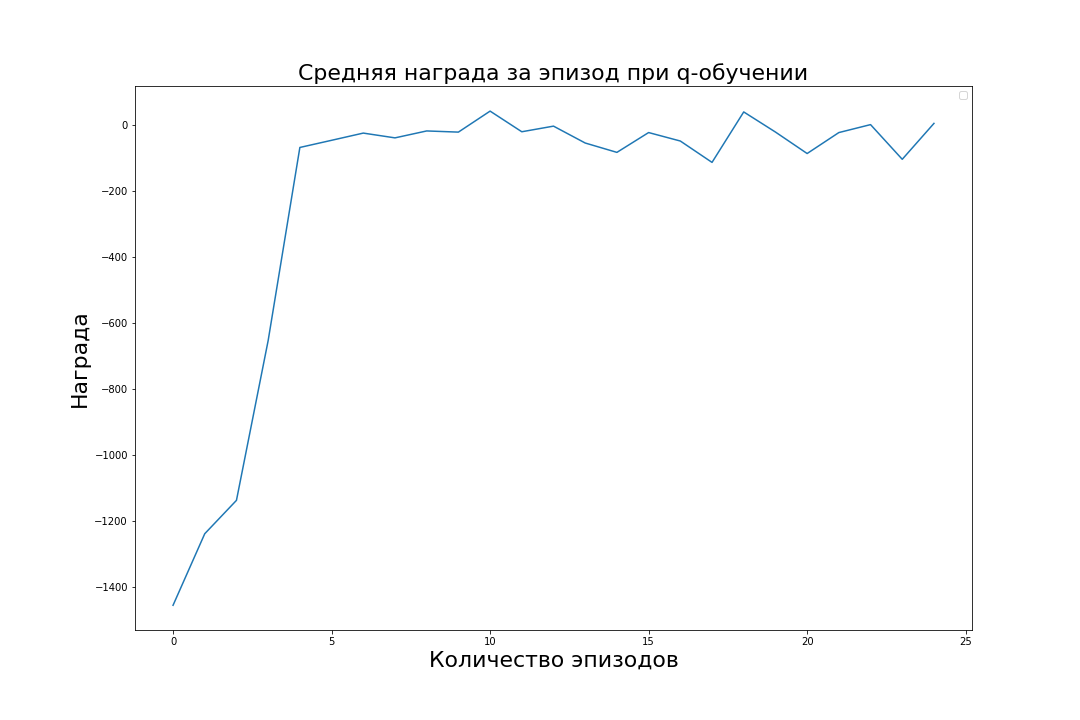
\includegraphics[scale=0.5]{rews.png}
	\label{fig:agent}
\end{figure}



%%%%%%%%%%%%%%%%%%%%%%%%%%%%%%%%%%%%%%%%%%%%%%%%%%%%%%%%%%%%%%%%%%%%%%%%%%%%%%%%
\section{Результаты метода MPC параллельно с обучением модели}\label{1sec:optimal-control}
%%%%%%%%%%%%%%%%%%%%%%%%%%%%%%%%%%%%%%%%%%%%%%%%%%%%%%%%%%%%%%%%%%%%%%%%%%%%%%%%

В рамках данной задачи согласно схеме из рисунка 3.3 мы обучали модель среды и параллельно запускали метод MPC для выбора следующего действия. Один эпизод длиться 200 итераций. В результате модель научилась довольно точно предсказывать следующее состояние среды. График ошибки состояния среды за 6 эпизодов по 200 действий представлен на рисунке 4.5. \newpage

\begin{figure}[!h]
	\caption {Абсолютная ошибка в состоянии среды}
	\centering
	\includegraphics[scale=0.35]{mpc_obs.png}
	\label{fig:agent}
\end{figure}

Кроме того наша модель среды научилась довольно точно предсказывать награду. График абсолютной ошибки предсказанной награды представлен на рисунке 4.6. \newpage

\begin{figure}[!h]
	\caption {Абсолютная ошибка в предсказании награды}
	\centering
	\includegraphics[scale=0.53]{mpc_rew_err.png}
	\label{fig:agent}
\end{figure}

График же ошибки нейронной сети (модели среды) по мере ее обучения каждые 10 итераций игры представлен ниже. Видно, что ошибка падает и модель среды все больше становится похожа непосредственно на среду. \newpage

\begin{figure}[!h]
	\caption {Абсолютная ошибка в предсказании награды}
	\centering
	\includegraphics[scale=0.4]{mpc_loss.png}
	\label{fig:agent}
\end{figure}

Реальная награда к тому же при помощи этих методов тоже растет внутри каждого эпизода. График ее роста можно увидеть ниже. \newpage

\begin{figure}[!h]
	\caption {Абсолютная награда}
	\centering
	\includegraphics[scale=0.6]{reward.png}
	\label{fig:agent}
\end{figure}



%%%%%%%%%%%%%%%%%%%%%%%%%%%%%%%%%%%%%%%%%%%%%%%%%%%%%%%%%%%%%%%%%%%%%%%%%%%%%%%%
\section{Результаты метода MPC на реальной среде и на претренированной }\label{1sec:optimal-control}
%%%%%%%%%%%%%%%%%%%%%%%%%%%%%%%%%%%%%%%%%%%%%%%%%%%%%%%%%%%%%%%%%%%%%%%%%%%%%%%%


Теперь попробуем сначала потренировать модель среды, генерируя действия рандомно и посмотрим даст ли нам это улучшений. Сначала посмотрим насколько точно предсказывается награда. \newpage


\begin{figure}[!h]
	\caption {Ошибка награды в предобученной модели. }
	\centering
	\includegraphics[scale=1]{ptretr_err.png}
	\label{fig:agent}
\end{figure}

Видно, что ошибка сильно скачет. Так что улучшений нам это не дало, но посмотрим на другие характеристики. Например на то, насколько быстро падает loss у нейронной сети модели среды. \newpage



\begin{figure}[!h]
	\caption {График loss нейронной сети для предобученной модели. }
	\centering
	\includegraphics[scale=0.25]{ptetr_loss.png}
	\label{fig:agent}
\end{figure}


Видно, что сходимость намного хуже. И еще проверим насколько хорошо работает MPC и получает высокую награду. 


\begin{figure}[!h]
	\caption {График loss нейронной сети для предобученной модели. }
	\centering
	\includegraphics[scale=0.85]{pretr_rew.png}
	\label{fig:agent}
\end{figure}

Видно, что по всем трем параметрам данный метод работает хуже, чем исходный. Поэтому в дальнейшем не будем предобучать модель среды на рандомной политике, а будем обучать ее непосредственно совместно с MPC.


%%%%%%%%%%%%%%%%%%%%%%%%%%%%%%%%%%%%%%%%%%%%%%%%%%%%%%%%%%%%%%%%%%%%%%%%%%%%%%%%
\section{Результаты метода MPC на реальной среде и сравнение}\label{1sec:optimal-control}
%%%%%%%%%%%%%%%%%%%%%%%%%%%%%%%%%%%%%%%%%%%%%%%%%%%%%%%%%%%%%%%%%%%%%%%%%%%%%%%%

Теперь попробуем применить метод MPC не для модели среды, а непосредственно на взаимодействии со средой. Получается, что итоговая награда будет расти. Ниже приведен график того, как MPC увеличивает награду на каждом шаге эпизода. 


\begin{figure}[!h]
	\caption {Награда на реальной среде}
	\centering
	\includegraphics[scale=0.8]{true.png}
	\label{fig:agent}
\end{figure}

Теперь сравним ее с наградой, которую получаем на претренированной модели. Как и ожидалось награда там выше, так как модель среды не до конца представляет среду. Хотя к концу они обе сходятся к 0. \newpage

\begin{figure}[!h]
	\caption {Награда на реальной среде}
	\centering
	\includegraphics[scale=0.4]{pretr_rew_com.png}
	\label{fig:agent}
\end{figure}

